\documentclass[12pt, twoside]{article}
\usepackage[francais]{babel}
\usepackage[T1]{fontenc}
\usepackage[latin1]{inputenc}
\usepackage[left=1cm, right=1cm, top=1cm, bottom=1cm]{geometry}
\usepackage{float}
\usepackage{graphicx}
\usepackage{array}
\usepackage{multirow}
\usepackage{amsmath,amssymb,mathrsfs}
\usepackage{soul}
\usepackage{textcomp}
\usepackage{eurosym}
 \usepackage{variations}
\usepackage{tabvar}

\pagestyle{empty}
\begin{document}

\section*{\center{Correction du devoir maison 1}}


\subsection*{Quelques erreurs}

\begin{tabular}{cc}
\begin{minipage}{10cm}

1)

 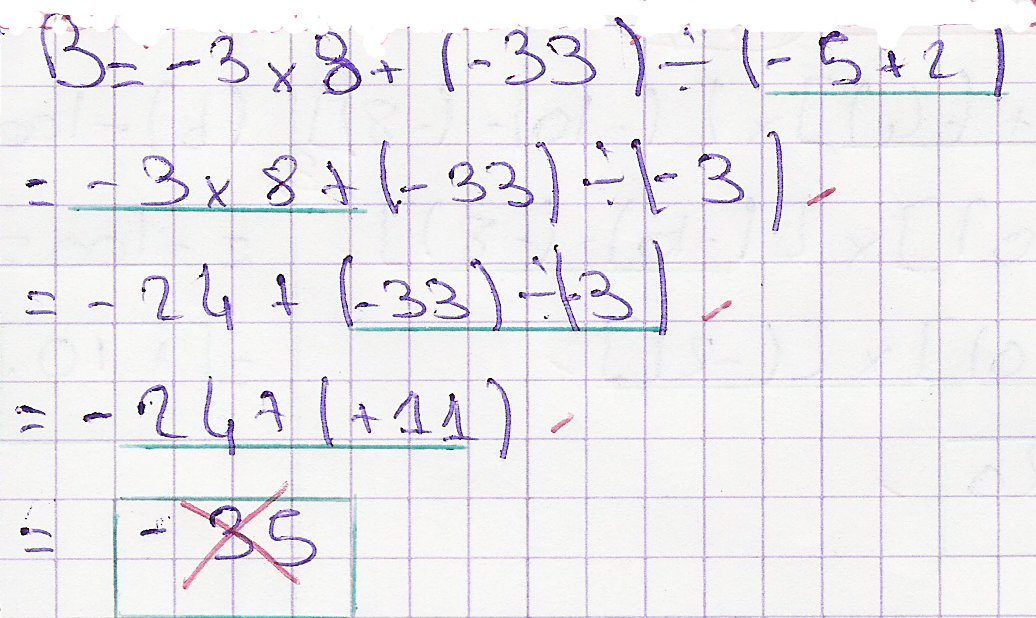
\includegraphics[width=6cm]{images/melanie.jpg}

\bigskip



 2) 
 
 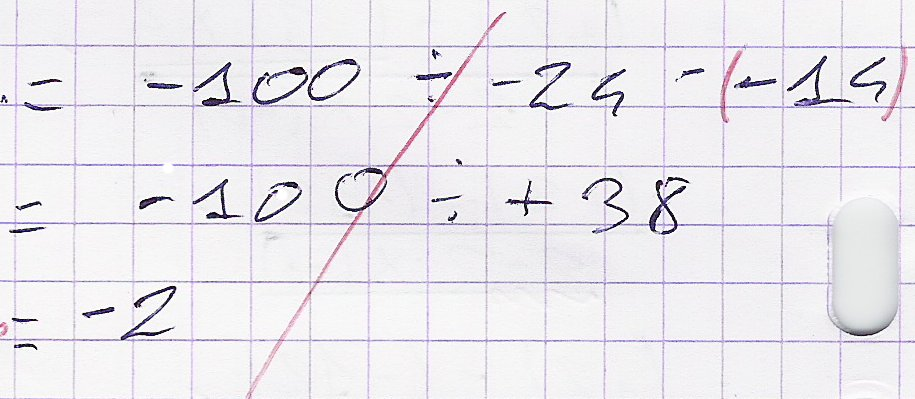
\includegraphics[width=6cm]{images/constance.jpg}
\end{minipage}
&
\begin{minipage}{8cm}

3)

 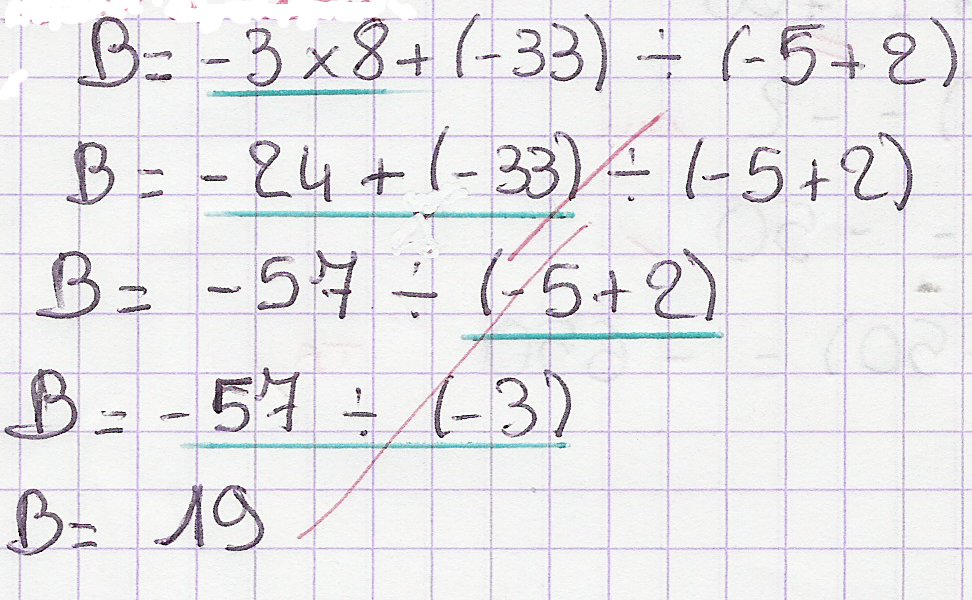
\includegraphics[width=6cm]{images/salma.jpg}


\bigskip

4)

 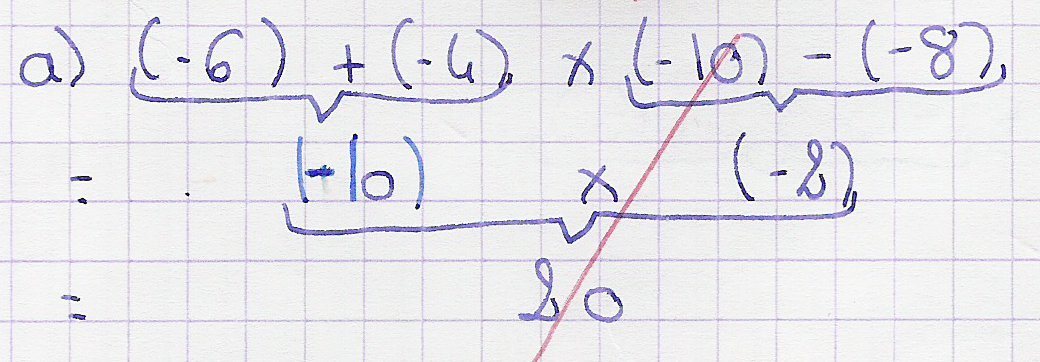
\includegraphics[width=6cm]{images/frank.jpg}


\end{minipage}
\end{tabular}

\bigskip

\bigskip

5) Effectuer le calcul suivant: $F=\dfrac{15+ \big( (-3) \times (-2)+(-5)
\big)}{-2 \times 7 - \big( (-6)+8 \times (-3) \big)}$

\enskip

D�but de r�ponse propos�e:
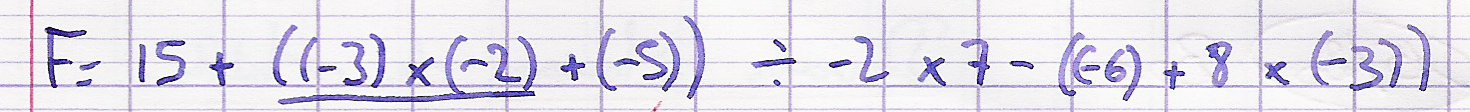
\includegraphics[width=10cm]{images/remi.jpg}



\bigskip

\bigskip

6) Traduire par un calcul: ``le quotient de -100 par la diff�rence de -24 et de
-14''.


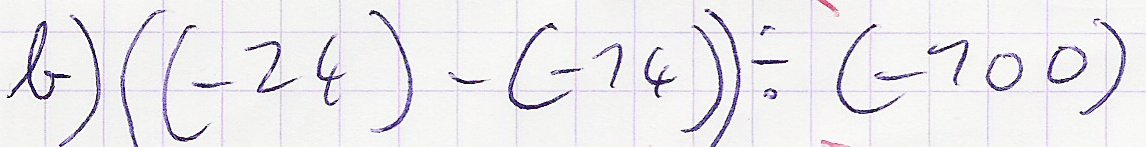
\includegraphics[width=7cm]{images/benjamin.jpg}

\subsection*{Exercice 1}

\begin{tabular}{cc}
\begin{minipage}{9cm}
$A=(-3) \times 5 +1 + (-2) \times (-2)$

$A=(-3) \times 5 +1 +4$

$A=-15 +1+4$

$A=-14+4$

$A=-10$

\enskip

$B= -3 \times 8 +(-33) \div (-5+2)$

$B= -3 \times 8 +(-33) \div (-3)$

$B= -24 +(-33) \div (-3)$

$B=-24+11$

$B=-13$
\end{minipage}
&
\begin{minipage}{9cm}
$C=11+2 \times \big( (-3)+(-7) \times 3 \big)$

$C=11+2 \times \big( (-3) +(-21) \big)$

$C=11+2 \times (-24)$

$C=11+ (-48)$

$C=-37$


\enskip

$D=(-14) \div (-7) + (-15) \div (+5)$

$D=(+2)+ (-15) \div (+5)$

$D=2+(-3)$

$D=-1$
\end{minipage}
\end{tabular}


\subsection*{Exercice 4}


$7 \times (-100)=-700$

$-3-(-5)=-3+(+5)=2$

$2 \times 25=50$

$-700+50=-650$

\end{document}
